\section{The Theory of nuclear forces}
Ever since it was discovered that the nucleus is made up from protons and neutrons, scientists have been working out how it is held together.
The logical answer would be a force, though the only two forces known at the time were the gravitational and the electromagnetic.
However, neither of these could be the one as protons and neutrons don't have opposite charges and the gravitational force is far too weak to explain the phenomenon.
% So it was concluded it must be another force, called the nuclear force, which we now know to be residual effects of the strong force between quarks, another fundamental force.
So it was concluded it must be another force, called the nuclear force. \cite{hergert_guided_2020, machleidt_chiral_2011}

% citing [1], [2] for "residual", possibly textbooks, it's kinda basic stuff

\subsection{Exchange particles and meson theories}
The first theory for the nuclear force was developed by Yukawa, introducing his exchange particles.
From an intuitive standpoint, the Heisenberg uncertainty principle allows for short term spontaneous creation of particles \cite{machleidt_nuclear_2013}.
These particles can then transfer momentum between two nucleons, by interactions, before vanishing again.
This mechanism does impose certain range and strength constraints on the force however, as a stronger force requires more massive exchange particles, giving them less time to exist and travel between nucleons \cite{machleidt_nuclear_2013, hergert_guided_2020}.

Yukawa predicted the properties of suitable exchange particles and when the pion and other suitable mesons were discovered they gave rise to so called meson theories. % 1950s
Many properties of simpler interactions were explained well with One Boson Exchange (OBE) models, where only one exchange of each meson is considered \cite{machleidt_nuclear_2013}.
However, adapting the theory for multiple exchanges wasn't as straight forward and led to the development of many more advanced models (Paris, Bonn, Stony Brook) \cite{machleidt_nuclear_2013, machleidt_meson_1989}.

\subsection{Quantum Chromodynamics}
Then Quantum Chromodynamics (QCD) was developed, quarks discovered and the strong force was introduced between them, mediated by gluons.
This completely changed the picture of the nuclear force, as the attraction of nucleons was now attributed to residuals of the strong force, delegating the meson theories to models.
However, calculating the nuclear force directly from QCD is very difficult for a variety of reasons, QCD is highly nonpertrubative at this range/scale making it is difficult to calculate and even a 2 nucleon interaction would already involve 6 quarks.
Still, attempts are made using finite step computer simulations, called Lattice QCD, which are very useful for verifying simple interactions but aren't suitable for regular day-to-day applications \cite{machleidt_nuclear_2013, hergert_guided_2020}.

\subsection{Effective Field Theory}
Applying Effective Field Theory (EFT) was the next break through, the key is that the significant effects may be studied independently at different scales.
To use EFT one must first identify the degrees of freedom (the interacting particles/entities), in our case nucleons and mesons (at the nucleon scale, mesons are the relevant exchange particles).
Then one constructs a Lagrangian (which is essentially an expression describing the dynamics of the system) in a certain way.
The key is to construct the most general possible Lagrangian that follows the same symmetries as the QCD strong force, as an expansion of $Q/\Lambda$.
Where $Q$ is the typical momentum of the system and $\Lambda$ the range at which the EFT interaction model stops being applicable.
The EFT application to QCD for modelling the nucleon interactions is called Chiral EFT (CEFT) as chirality (symmetry under reflection) is a key symmetry of the strong force \cite{machleidt_chiral_2011, machleidt_nuclear_2013, burgess_introduction_2007, hergert_guided_2020}.

Using CEFT is a rather involved process but the following tries to provide a short outline of the key features.
There are 2 main decisions, the first being how many nucleons do we include, the simplest being 2 nucleons (NN), following with 3 nucleons (3N), 4 nucleons (4N) and many nucleons.
The second is how many terms of the mentioned expansion do we take into account, these simplest here is regarded as the Leading Order (LO) followed by Next Leading Order (NLO), Next Next Leading Order (NNLO) and so on.
Determining both of these specifies which interactions need to be considered, \cref{fig:diagram1} shows Feynman diagrams for some.
In these there are different types of nodes each associated with a Low Energy Constant (LEC) which are determined by fitting experimental data and influence how the interaction affects the force \cite{machleidt_chiral_2011, machleidt_nuclear_2013, burgess_introduction_2007, hergert_guided_2020}.

\subsection{Nuclear Shell Theory}
The nuclear shell model originates from scientists observing that atoms with certain numbers of protons and neutrons (called magic numbers, covered more later) were more stable than others, which resembled the effects of shell closures in the atomic shell model.
Simplest shell models consider the individual nucleons to behave independently, each in a potential formed by the many NN interactions, where this potential results in a central potential with additional spin-orobit, spin-spin and tensor components \cite{kruecken_introduction_2011}.

\begin{figure}[H]
    \centering
    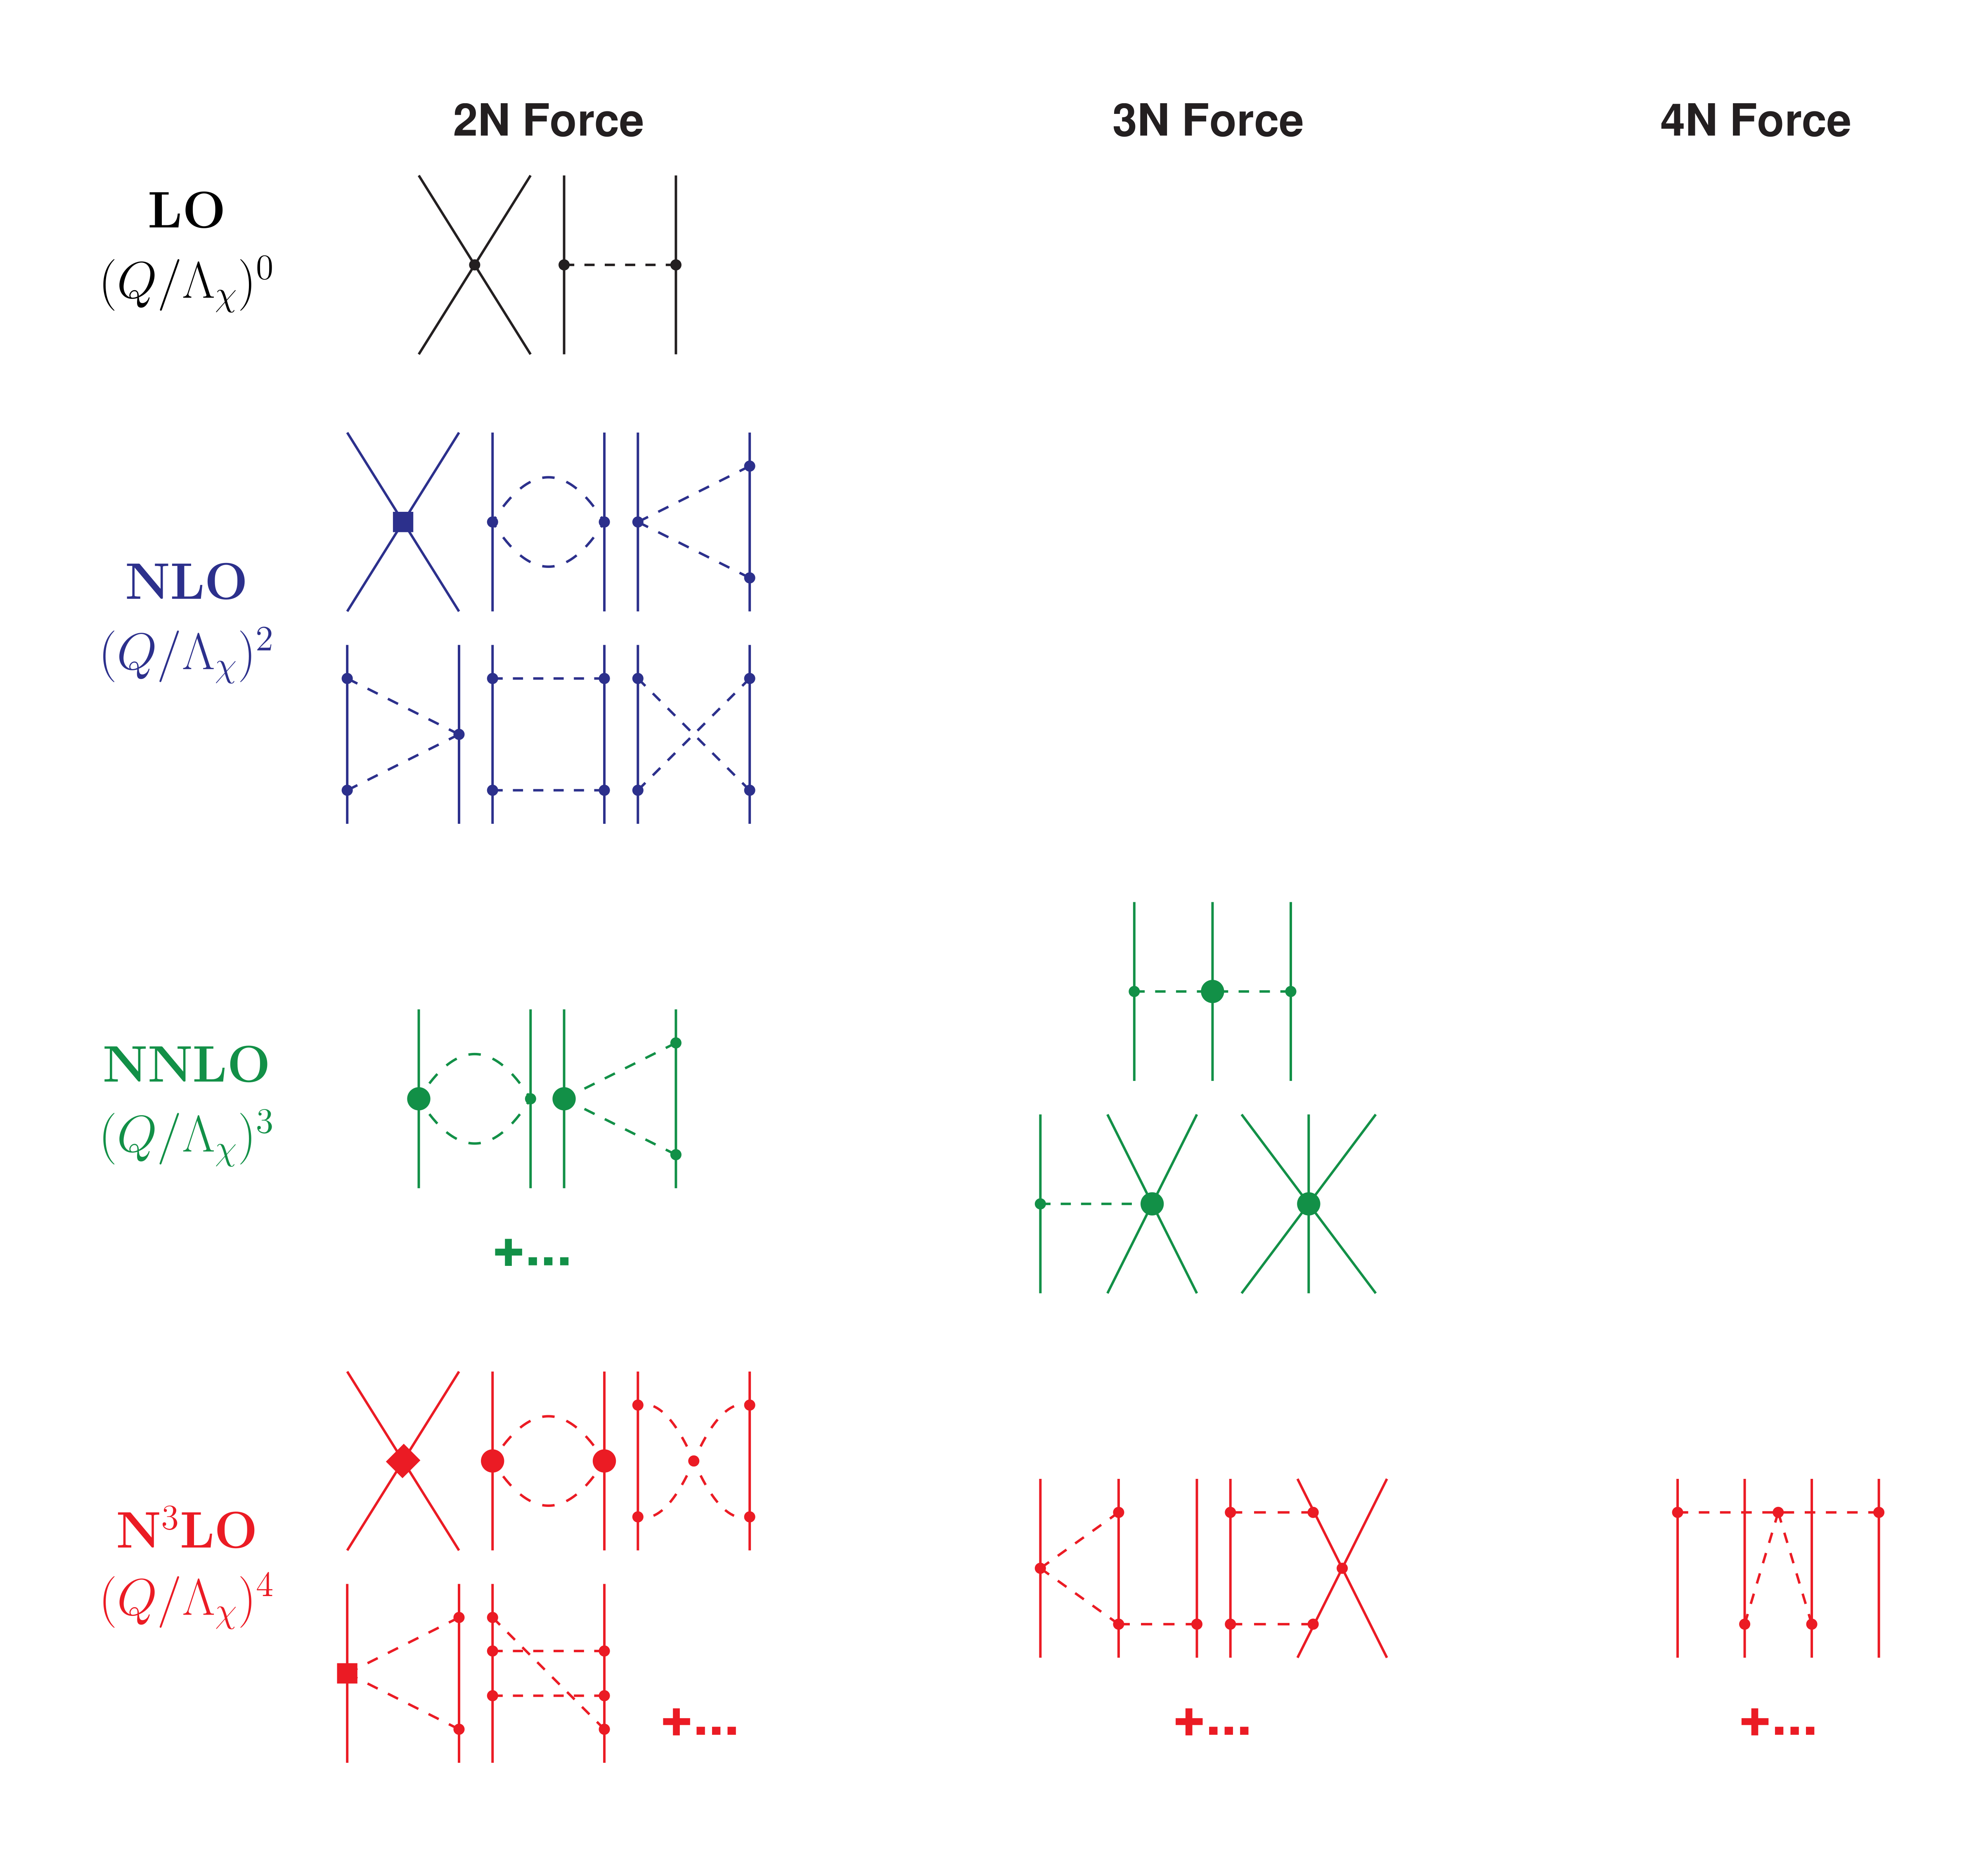
\includegraphics[width=.4\textwidth]{images/NFthe_diagram.png}
    \caption{Feynman diagrams showing some of the first interactions that need to be considered when using CEFT. Solid lines represent nucleons and dashed lines pions. Different nodes represent different interactions \cite{machleidt_chiral_2011}.}\label{fig:diagram1}
\end{figure}

% The Nuclear Shell Model concerns the nuclear force from a different perspective, it is based on experimental observations made around the 1940s.
% Scientists have observed that atoms that have certain numbers of protons or neutrons are more stable (called the magic numbers and covered more in the following sections).
% These were taken as evidence for shell closures similar to those in the shell model of the atom, thus nuclear shell theory started.
% The underlying idea is that the nucleons within the nucleus move almost independently of each other, 

\subsection{Outlook}
Finally, for a general outlook, most stable nuclei (especially ones in the valley of stability) are modeled well using combinations of the meson theories, CEFT based nuclear shell models (NN is often sufficient for stable isotopes) and other approaches.
However for exotic, neutron-rich nuclei the models fall short, at least 3N interactions need to be considered \iffalse cite Wienholtz \fi for an accurate model and more measurements are currently being made.
% However, most of the models fall short in some way, some need to be localized to be accurate enough, some are too computationally expensive to carry out for heavy isotopes and so on.
% After it was determined that for 
% Currently much work is being done on expending the CEFT approaches to contain more complicated nucleon

% Applying Effective Field Theory (EFT) was the next break through, EFT is somewhat similar to multipole expansion of electromagnetism. % cite the presentation
% The key is that the significant effects may be studied independently at different scales, to use EFT one must first identify the degrees if freedom (the interacting particles/entities), in our case nucleons and mesons.

% Applying Effective Field Theory (EFT) was the next break through, EFT is somewhat similar to multipole expansion of electromagnetism. % cite the presentation
% The key is that the effects of the strong force at the nucleon scale may be modeled without full understanding of all the details.
% EFT is a quantum theory and 

% cite [10]

% Applying Effective Field Theory (EFT) was the next break through, it allows approximating the QCD effects on a nucleon level.


